\section{Grafici ed immagini}

\begin{figure}[h]
	\centering
	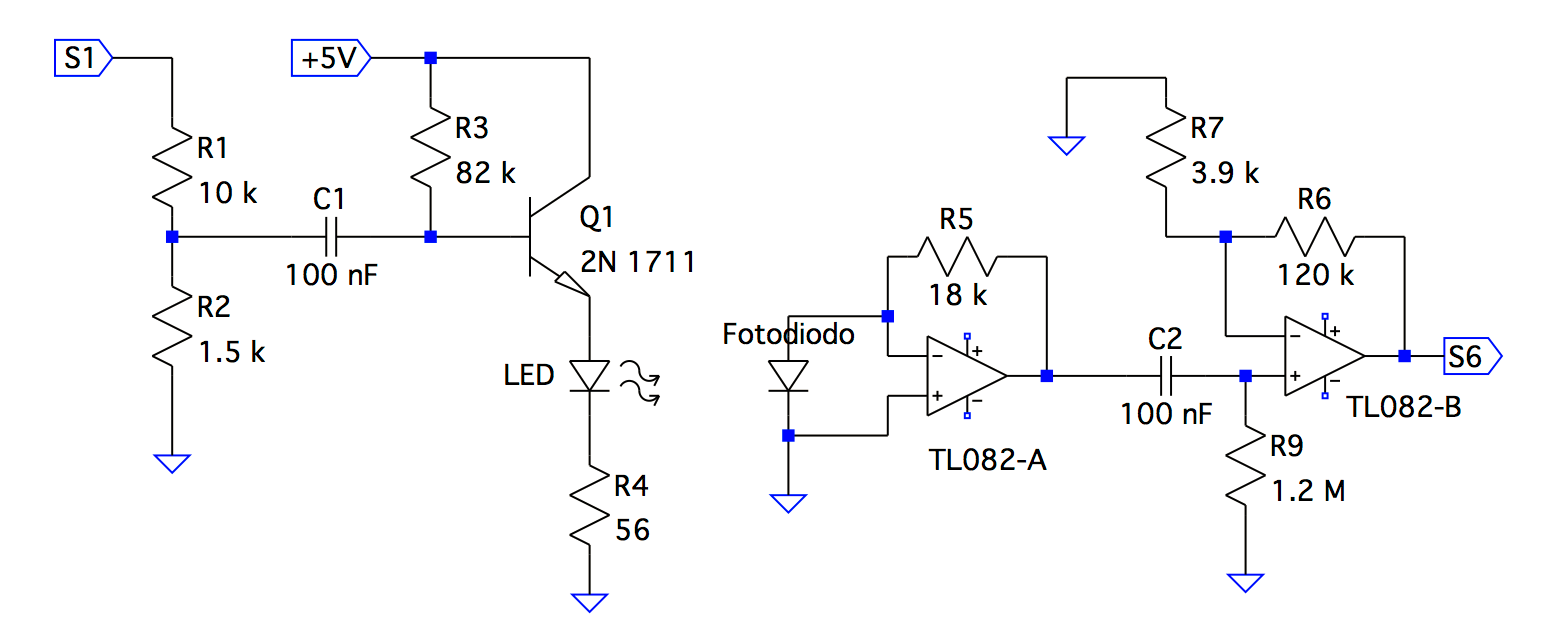
\includegraphics[scale=0.4]{amplificatore_potenza.png}
	\caption{Schema circuitale di amplificatore di potenza e pre-amplificatore.}
	\label{f:pre-amp}
\end{figure}

\begin{figure}[h]
	\centering
	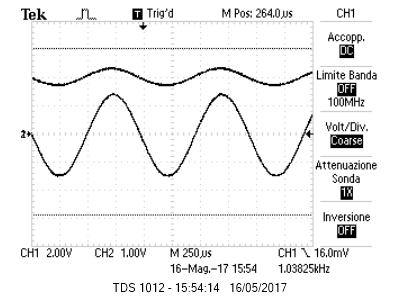
\includegraphics[scale=0.9]{amplpotenza.png}
	\caption{Segnale in ingresso (mostrato inferiormente) e segnale in uscita all'emettitore del transistor Q1 (sopra).}
	\label{f:amplpotenza}
\end{figure}

\begin{figure}[h]
	\centering
	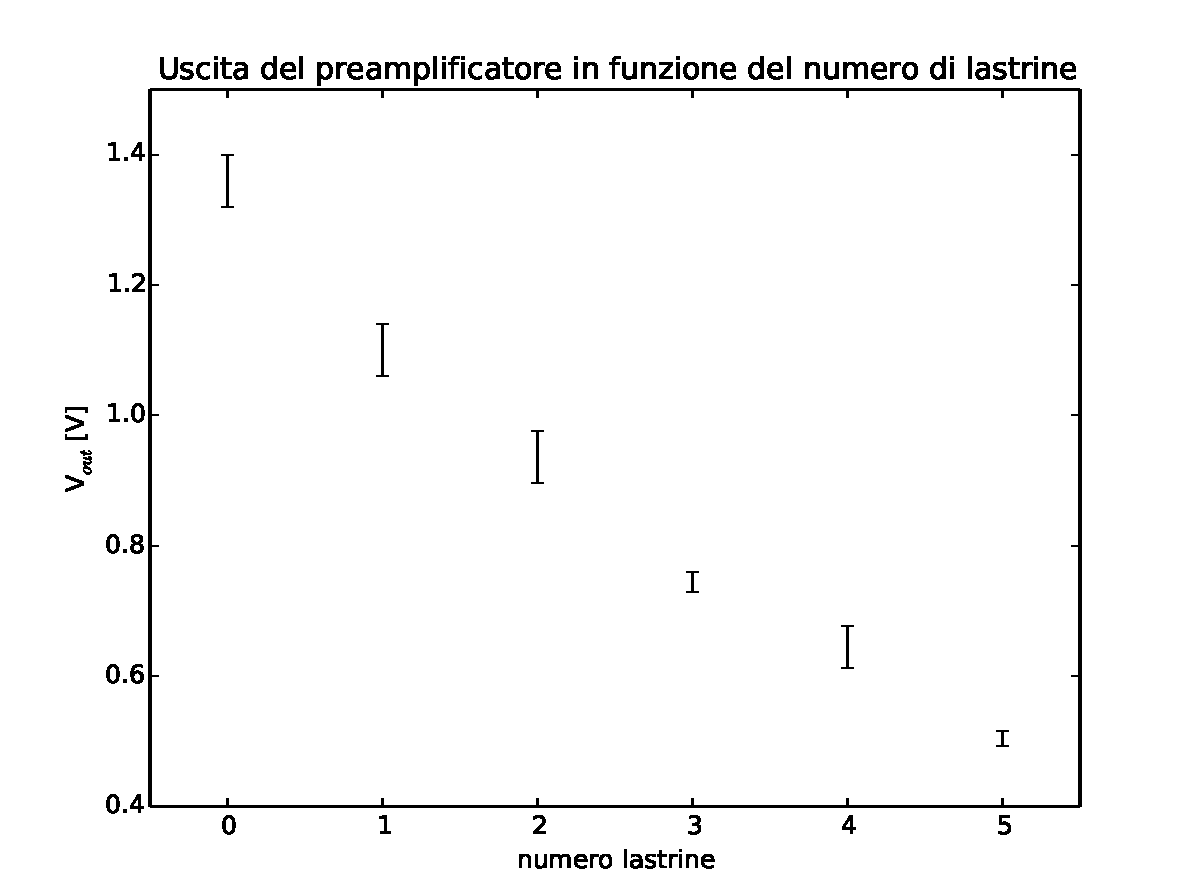
\includegraphics[scale=0.7]{grafico1.pdf}
	\caption{Grafico dell'ampiezza dell'uscita del pre-amplificatore, misurata all'oscilloscopio con errore di lettura, in funzione del numero di lastrine.}
	\label{f:Grafico1}
\end{figure}

\begin{figure}[h]
	\centering
	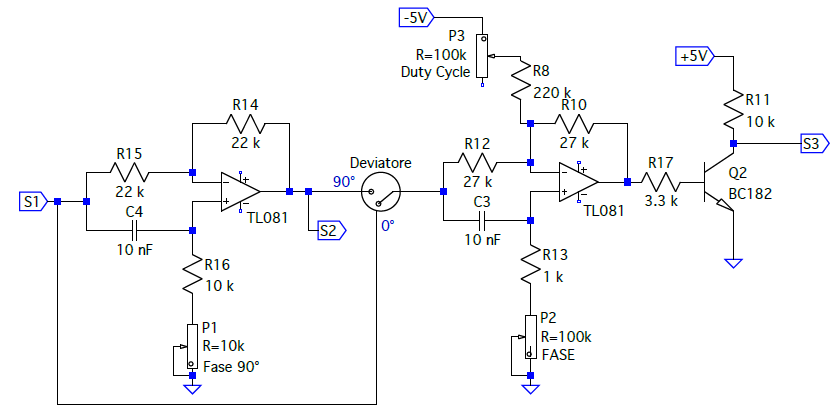
\includegraphics[scale=0.7]{adattamento_fase.png}
	\caption{Schema del circuito degli sfasatori, di 90$^\circ$ e a fase variabile, che permettono l'adattamento di fase.}
	\label{f:adattamento_fase}
\end{figure}

\begin{figure}[h]
	\centering
	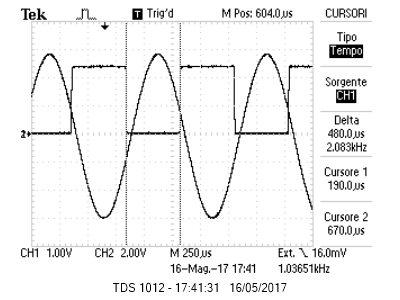
\includegraphics[scale=0.9]{S3-S1deviatore0.png}
	\caption{Segnale in S3 (onda quadra) ed in S1 (onda sinusoidale) con deviatore nella posizione 0$^\circ$.}
	\label{f:S3-S1deviatore0}
\end{figure}

\begin{figure}[h]
	\centering
	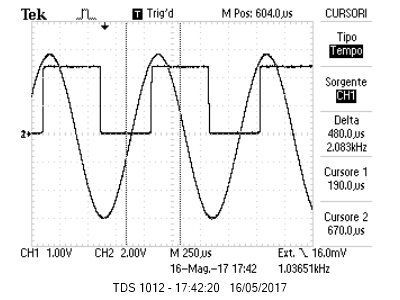
\includegraphics[scale=0.9]{S3-S1deviatore90.png}
	\caption{Segnale in S3 (onda quadra) ed in S1 (onda sinusoidale) con deviatore nella posizione 90$^\circ$.}
	\label{f:S3-S1deviatore90}
\end{figure}

\begin{figure}[h]
	\centering
	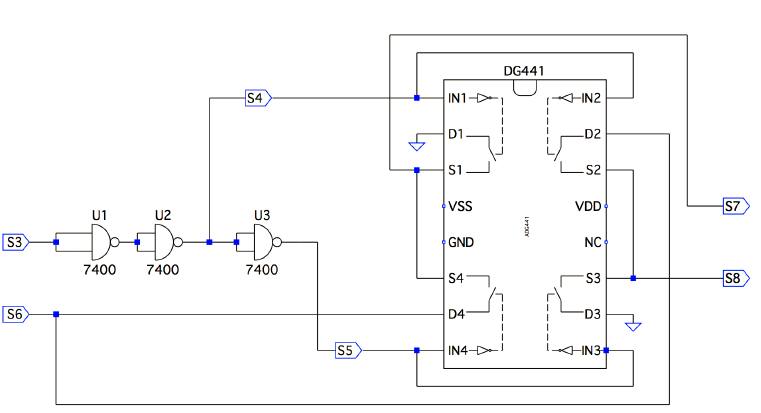
\includegraphics[scale=0.7]{squadratore.png}
	\caption{Schema del circuito per squadratore e campionatore.}
	\label{f:squadratore}
\end{figure}

\begin{figure}[h]
	\centering
	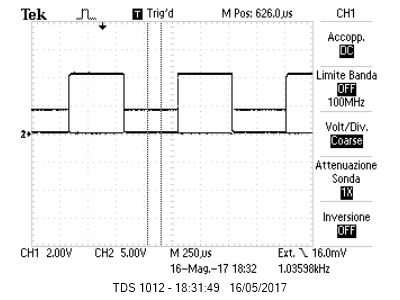
\includegraphics[scale=0.9]{s4-s5.png}
	\caption{Segnali logici nelle posizioni S4 ed S5. Si può verificare che i segnali sono complementari, ovvero in opposizione di fase.}
	\label{f:s4-s5}
\end{figure}

\begin{figure}[h]
	\centering
	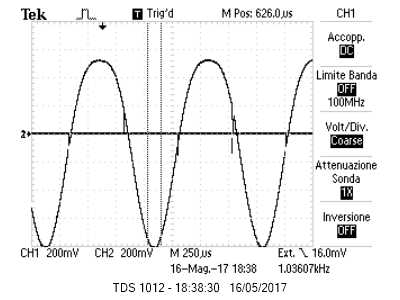
\includegraphics[scale=0.9]{S7-8deviatore0.png}
	\caption{Segnale in S7 ed in S8 con deviatore nella posizione 0$^\circ$.}
	\label{f:S7-8deviatore0}
\end{figure}

\begin{figure}[h]
	\centering
	\includegraphics[scale=0.9]{S7-8-deviatore90.png}
	\caption{Segnale in S7 ed in S8 con deviatore nella posizione 90$^\circ$.}
	\label{f:S7-8deviatore90}
\end{figure}

\begin{figure}[h]
	\centering
	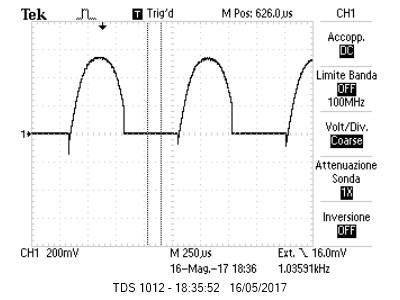
\includegraphics[scale=0.9]{S7deviatore0.png}
	\caption{Segnale in S7 con deviatore nella posizione 0$^\circ$.}
	\label{f:S7deviatore0}
\end{figure}

\begin{figure}[h]
	\centering
	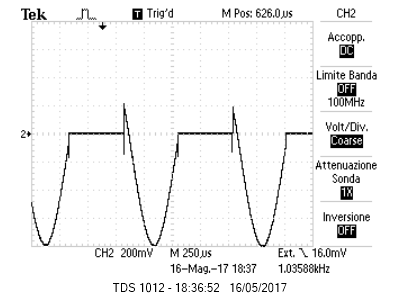
\includegraphics[scale=0.9]{S8deviatore0.png}
	\caption{Segnale in S8 con deviatore nella posizione 0$^\circ$.}
	\label{f:S8deviatore0}
\end{figure}

\begin{figure}[h]
	\centering
	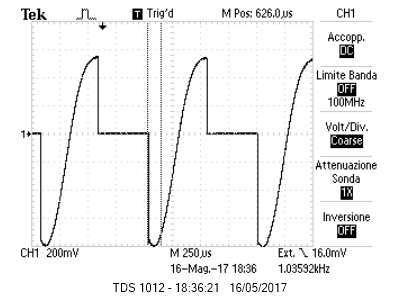
\includegraphics[scale=0.9]{S7deviatore90.png}
	\caption{Segnale in S7 con deviatore nella posizione 90$^\circ$.}
	\label{f:S7deviatore90}
\end{figure}



\begin{figure}[h]
	\centering
	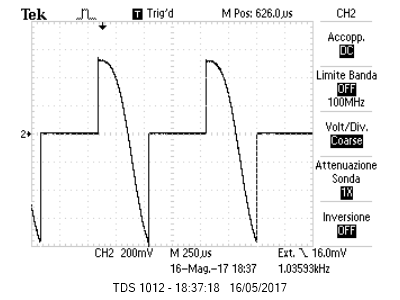
\includegraphics[scale=0.9]{S8deviatore90.png}
	\caption{Segnale in S8 con deviatore nella posizione 90$^\circ$.}
	\label{f:S8deviatore90}
\end{figure}

\begin{figure}[h]
	\centering
	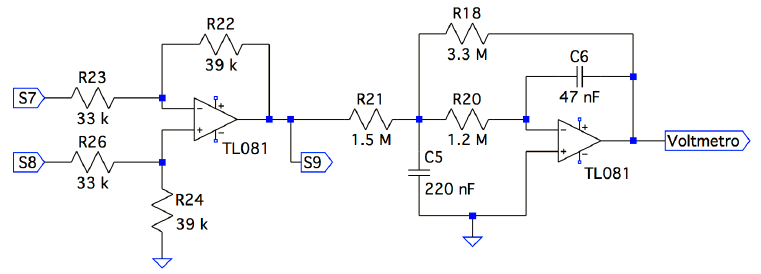
\includegraphics[scale=0.9]{mediatore.png}
	\caption{Schema di amplificatore differenziale(prima di S9) e mediatore.}
	\label{f:Mediatore}
\end{figure}

\begin{figure}[h]
	\centering
	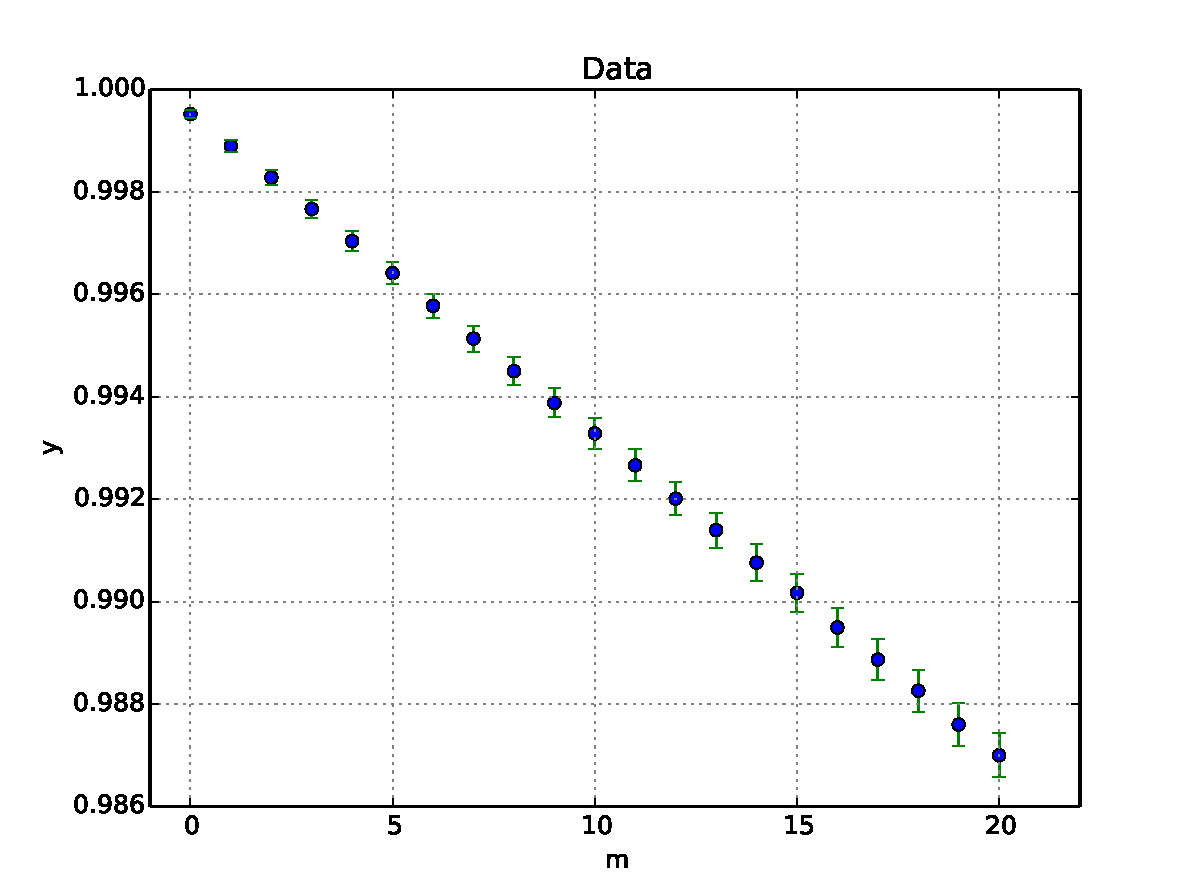
\includegraphics[scale=0.7]{grafico.pdf}
	\caption{Fit di $V_{out}$ in funzione del numero di lastrine. Sotto è mostrato il grafico dei residui. Il fit eseguito è a 2 parametri.}
	\label{f:Grafico}
\end{figure}
\begin{figure}[h]
	\centering
	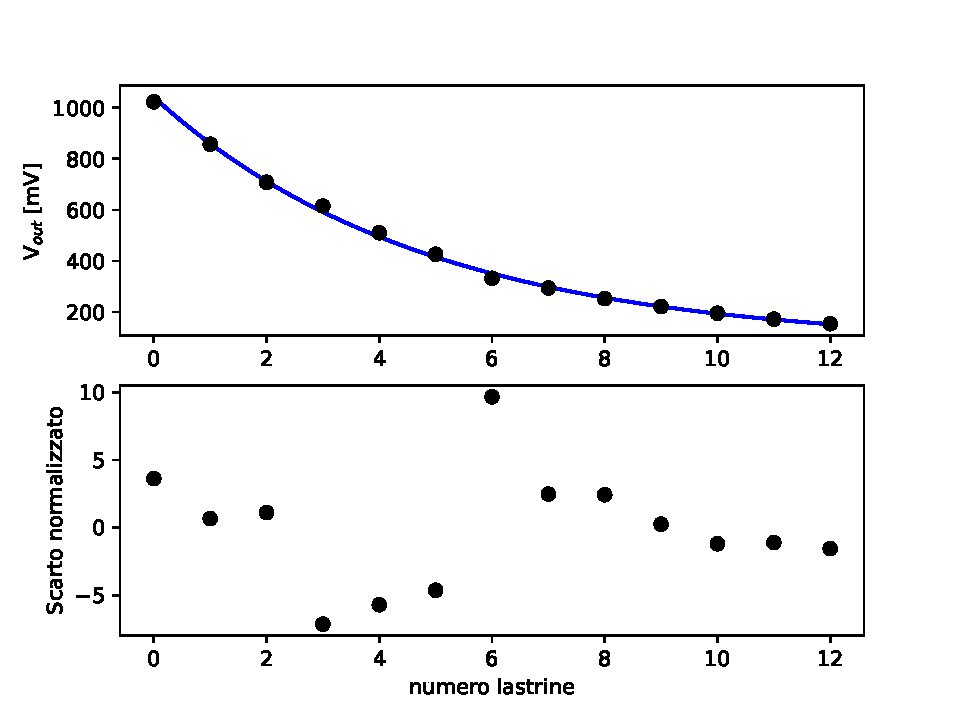
\includegraphics[scale=0.7]{grafico4.pdf}
	\caption{Fit di $V_{out}$ in funzione del numero di lastrine. Sotto è mostrato il grafico dei residui, che non sembra evidenziare andamenti sistematici. In tal caso il fit è a 3 parametri, con aggiunta dell'offset.}
	\label{f:Grafico4}
\end{figure}